%%%%%%%%%%%%%%%%%%%%%%%%%%%%%%%%%%%%%%%%%%%%%%%%%%%%%%%%%%%%%%%%%%%%%%
% Skupina30/main.tex
%
% Pravila predloge:
%  - brez \usepackage (vse pakete naloži editor.tex),
%  - slike v Skupina30/img/, vse oznake in ključi virov z "g30:",
%  - vire dodajte v skupno datoteko references.bib (z doi ali url).
%%%%%%%%%%%%%%%%%%%%%%%%%%%%%%%%%%%%%%%%%%%%%%%%%%%%%%%%%%%%%%%%%%%%%%

\graphicspath{{Skupina30/img/}}

\title{Koliko kubitov lahko prepletemo? Vpliv tehnik za blaženje napak na zvestobo stanj GHZ na kvantnem procesorju IBM}
\titlerunning{Koliko kubitov lahko prepletemo?}
\author{Veno Jakomin, Jure Pahor in Grega Potočnik}
\maketitle

\abstract{Stanje GHZ preplete vse kubite naenkrat, zato je občutljiv pokazatelj zmogljivosti kvantnega procesorja, zvestoba nad $0{,}5$ pa dokazuje pristno večdelno prepletenost. Zanimalo nas je, pri kolikšnem številu kubitov procesor IBM to mejo še doseže in koliko jo premaknejo dinamično razklapljanje, Paulijevo sukanje in ekstrapolacija na ničelni šum. Stanje smo pripravili z linearno verigo vrat CNOT in z drevesom BFS, zvestobo pa izmerili iz populacij in paritetnih nihanj. Na procesorju \texttt{ibm\_fez} je drevo s samim popravkom napak branja doseglo pristno prepletenost pri 40 kubitih, veriga pa pri 16. Razklapljanje in sukanje sta mejo drevesa znižala na največ 32 kubitov, ekstrapolacija pa je porabo procesorskega časa skoraj podvojila (\SI{123}{\second} proti \SI{64}{\second}). Rezultat kaže, da je bila na tej napravi za doseg prepletenosti pomembnejša plitvost vezja kot vklop tehnik za blaženje napak.}


\section{Uvod}
\label{g30:sec:uvod}

Prepletenost je eden ključnih virov kvantnega računanja~\cite{nielsen2010}, zato je priprava prepletenih stanj na čim večjem številu kubitov pogost preizkus kakovosti kvantnega procesorja. Današnje naprave so pri tem omejene s šumom: vrata niso popolna, kubiti se relaksirajo in defazirajo, branje stanja pa se zmoti pri približno enem odstotku meritev~\cite{preskill2018}.

Za preizkus prepletenosti se uporablja stanje GHZ,
\begin{equation}
\ket{\mathrm{GHZ}_n} = \frac{1}{\sqrt{2}}\left(\ket{0}^{\otimes n} + \ket{1}^{\otimes n}\right),
\label{g30:eq:ghz}
\end{equation}
pri katerem so vsi kubiti hkrati v stanju \enquote{vse ničle} in \enquote{vse enice}. Dovolj je, da se defazira en sam kubit, in relativna faza med obema členoma je izgubljena; če je verjetnost defaziranja na kubit enaka $p$, koherenca pada kot $(1-2p)^n$.

Zvestoba $F = \bra{\mathrm{GHZ}}\rho\ket{\mathrm{GHZ}}$ nad $1/2$ je zadosten pogoj za pristno večdelno prepletenost (GME)~\cite{g30:guhne2009}, oceni pa se iz populacij obeh robnih izidov in iz amplitude paritetnih nihanj~\cite{g30:monz2011}. Na procesorjih IBM so Kam in sod.\ brez detekcije napak potrdili GME pri 32 kubitih~\cite{g30:kam2024}, Javadi-Abhari in sod.\ pa z detekcijo napak in post-selekcijo pri 120 kubitih~\cite{g30:bigcats2025}. Obe skupini sta uporabili plitvejša vezja od naivne verige vrat CNOT.

V teh objavah ni razčlenjena cena. Qiskit Runtime~\cite{qiskit2024} ponuja dinamično razklapljanje~\cite{g30:ezzell2023}, Paulijevo sukanje~\cite{g30:wallman2016} in ekstrapolacijo na ničelni šum~\cite{temme2017} kot nastavitve, ki jih uporabnik preprosto vklopi, vsaka pa porabi dodaten procesorski čas, ki je v brezplačnem načrtu IBM Quantum Open Plan omejen na deset minut na račun. Ekstrapolacija poleg tega poda oceno in ne meritve, zato lahko negotovost rezultata poveča bolj, kot izboljša njegovo vrednost.

\begin{svgraybox}
\textbf{Raziskovalno vprašanje.} Pri kolikšnem največjem številu kubitov $n_{\mathrm{max}}$ procesor IBM pripravi stanje GHZ z zvestobo $F > 0{,}5$ in za koliko ter za kakšno ceno v procesorskem času to mejo premaknejo dinamično razklapljanje, Paulijevo sukanje in ekstrapolacija na ničelni šum?

\textbf{Pričakovani rezultat.} S samim popravkom napak branja bo GME izgubljena pri približno 15--25 kubitih, razklapljanje in sukanje bosta $n_{\mathrm{max}}$ povečala za vsaj 30~\% za ceno večkratnega procesorskega časa. Ekstrapolacija bo ocenjeno zvestobo še povečala, a lahko zaradi večje negotovosti po pravilu $F - 2\sigma > 0{,}5$ mejo celo zmanjša. Plitvejše drevo BFS bo doseglo večji $n_{\mathrm{max}}$ kot linearna veriga vrat CNOT.
\end{svgraybox}

V Razdelku~\ref{g30:sec:metode} opišemo vezji, merjenje zvestobe, konfiguracije blaženja napak in izvedbo na procesorju. Razdelek~\ref{g30:sec:rezultati} podaja zvestobe na simulatorjih in procesorju, Razdelek~\ref{g30:sec:razprava} odgovor na raziskovalno vprašanje, vzrok za razliko med oblikama vezja in neuspele poskuse, Razdelek~\ref{g30:sec:zakljucek} pa povzetek in nadaljnje delo.


\section{Metode}
\label{g30:sec:metode}

\subsection{Orodja in nastavitve}
\label{g30:sec:orodja}

Vezja smo pripravili in izvedli v Qiskitu~\cite{qiskit2024} na procesorju \texttt{ibm\_fez} iz družine Heron~r2 s 156 kubiti, simulirali pa na njegovem odlitku \texttt{FakeFez}, ki vsebuje kalibracijske podatke prave naprave. Nastavitve, ki vplivajo na rezultat, so v Tabeli~\ref{g30:tab:parametri}.

\begin{table}[htbp]
\caption{Orodja in nastavitve poskusa.}
\label{g30:tab:parametri}
\centering
\setlength{\aboverulesep}{0pt}
\setlength{\belowrulesep}{0pt}
\renewcommand{\arraystretch}{1.2}
\begin{tabularx}{\textwidth}{|@{}>{\hspace{5pt}}l@{\hspace{5pt}}|@{\hspace{5pt}}>{\raggedright\arraybackslash}X@{\hspace{5pt}}|}
\toprule
Parameter & Vrednost \\
\midrule
procesor & \texttt{ibm\_fez} (Heron r2, 156 kubitov), odlitek \texttt{FakeFez} \\
orodja & Python 3.12, Qiskit 2.6.2, Aer 0.18.4, IBM Runtime 0.52.1, mthree 3.0.0 \\
prevajanje in simulacija & matrični produktni zapis stanja (MPS), stopnja optimizacije 1 \\
ponovitve meritve & 4096 (idealni simulator), 1024 (šumni); na procesorju 4096 za populaciji, 512 na fazo za koherenco in 1024 za kalibracijo mthree \\
koherenca & $2n+2$ faz, faktorji ojačanja šuma 1, 3, 5 \\
razklapljanje & zaporedje XY4 \\
\bottomrule
\end{tabularx}
\end{table}

Mediana napake branja je na tej napravi $7{,}6 \cdot 10^{-3}$, zato je pri 120 kubitih verjetnost pravilnega branja vseh kubitov le $(1-0{,}0076)^{120} \approx 0{,}40$ in popravek napak branja obravnavamo kot del osnovne konfiguracije.

\subsection{Priprava stanja GHZ in izbira kubitov}
\label{g30:sec:vezja}

Stanje~\eqref{g30:eq:ghz} smo pripravili na dva načina (Slika~\ref{g30:fig:vezji}). Linearna veriga na prvi kubit da vrata $H$ in nato z $n-1$ zaporednimi vrati CNOT superpozicijo prenese po verigi, zato globina raste z $n$. Drevo superpozicijo širi po drevesu BFS na grafu povezav procesorja, vrata, ki ne delijo kubitov, pa izvede vzporedno. Koren drevesa je kubit z najmanjšo ekscentričnostjo v izbranem podgrafu~\cite{g30:bigcats2025}, zato je globina drevesa enaka polmeru podgrafa. V vsaki plasti vsak kubit nastopa največ enkrat, otroke pa obdelamo po padajoči velikosti poddrevesa, da se najdaljša veja začne čim prej.

\begin{figure}[htbp]
\centering
\begin{subfigure}[b]{0.48\textwidth}
\centering
\resizebox{\linewidth}{!}{%
\begin{quantikz}
\lstick{$\ket{0}$} & \gate{H} & \ctrl{1} & \qw      & \qw      & \qw      & \qw \\
\lstick{$\ket{0}$} & \qw      & \targ{}  & \ctrl{1} & \qw      & \qw      & \qw \\
\lstick{$\ket{0}$} & \qw      & \qw      & \targ{}  & \ctrl{1} & \qw      & \qw \\
\lstick{$\ket{0}$} & \qw      & \qw      & \qw      & \targ{}  & \ctrl{1} & \qw \\
\lstick{$\ket{0}$} & \qw      & \qw      & \qw      & \qw      & \targ{}  & \qw
\end{quantikz}}
\caption{veriga}
\label{g30:fig:veriga}
\end{subfigure}
\hfill
\begin{subfigure}[b]{0.48\textwidth}
\centering
\resizebox{\linewidth}{!}{%
\begin{quantikz}
\lstick{$\ket{0}$} & \gate{H} & \ctrl{1} & \ctrl{2} & \qw      & \qw     & \qw \\
\lstick{$\ket{0}$} & \qw      & \targ{}  & \qw      & \ctrl{2} & \qw     & \qw \\
\lstick{$\ket{0}$} & \qw      & \qw      & \targ{}  & \qw      & \ctrl{2}& \qw \\
\lstick{$\ket{0}$} & \qw      & \qw      & \qw      & \targ{}  & \qw     & \qw \\
\lstick{$\ket{0}$} & \qw      & \qw      & \qw      & \qw      & \targ{} & \qw
\end{quantikz}}
\caption{drevo}
\label{g30:fig:drevo}
\end{subfigure}
\caption{Priprava stanja GHZ za $n = 5$. Pri verigi~(a) se vrata izvajajo zaporedno, zato je globina sorazmerna s številom kubitov. Pri drevesu~(b) so vrata zaradi preglednosti narisana zaporedno, v izvedbi pa se vrata iste plasti izvedejo vzporedno: najprej $\{(0,1)\}$, nato $\{(0,2), (1,3)\}$ in nazadnje $\{(2,4)\}$, zato je globina enaka globini drevesa in ne številu kubitov.}
\label{g30:fig:vezji}
\end{figure}

Graf povezav smo utežili z izmerjenimi napakami, povezave z napako vrat \texttt{cz} in vozlišča z napako branja. Za drevo iščemo povezan podgraf $n$ kubitov z najmanjšo vsoto uteži s pohlepno rastjo po Primovem načelu, za verigo pa pot z iskanjem v globino z vračanjem. Obe obliki imata $n-1$ dvokubitnih vrat in ne potrebujeta zamenjav SWAP, globina pa se bistveno razlikuje (Tabela~\ref{g30:tab:vezja}): pri 120 kubitih ima prevedena veriga globino 479, drevo pa 84, zato stanje v verigi obstaja približno \SI{11}{\micro\second}, v drevesu pa \SI{2}{\micro\second}.

\begin{table}[htbp]
\caption{Lastnosti vezij pred prevajanjem in po prevajanju na \texttt{ibm\_fez} pri stopnji optimizacije 1. Število dvokubitnih vrat je enako pri obeh oblikah, globina pa ne.}
\label{g30:tab:vezja}
\centering
\setlength{\aboverulesep}{0pt}
\setlength{\belowrulesep}{0pt}
\renewcommand{\arraystretch}{1.2}
\begin{tabularx}{\textwidth}{|@{}>{\hspace{5pt}}l@{\hspace{5pt}}|@{}>{\hspace{5pt}}r@{\hspace{5pt}}|>{\centering\arraybackslash}X>{\centering\arraybackslash}X|>{\centering\arraybackslash}X>{\centering\arraybackslash}X|}
\toprule
\multirow{2}{*}{Oblika} & \multirow{2}{*}{$n$} & \multicolumn{2}{c|}{pred prevajanjem} & \multicolumn{2}{c|}{po prevajanju} \\
\cline{3-6}
 & & CNOT & globina & CZ & globina \\
\midrule
\multirow{2}{*}{drevo} & 20 & 19 & 8 & 19 & 27 \\
 & 120 & 119 & 22 & 119 & 84 \\
\midrule
\multirow{2}{*}{veriga} & 20 & 19 & 20 & 19 & 79 \\
 & 120 & 119 & 120 & 119 & 479 \\
\bottomrule
\end{tabularx}
\end{table}

\subsection{Merjenje zvestobe}
\label{g30:sec:zvestoba}

Zvestobo stanja GHZ sestavljata dva dela,
\begin{equation}
F = \frac{1}{2}\left(P_{0\ldots0} + P_{1\ldots1}\right) + \frac{1}{2}C,
\label{g30:eq:zvestoba}
\end{equation}
kjer sta $P_{0\ldots0}$ in $P_{1\ldots1}$ verjetnosti obeh robnih izidov, $C = 2\left|\rho_{0\ldots0,\,1\ldots1}\right|$ pa koherenca~\cite{g30:monz2011, g30:wei2020}. Populaciji izmerimo v bazi $Z$, sami pa ne ločita superpozicije od klasične mešanice obeh izidov; za to je potrebna koherenca. Dobimo jo iz paritetnih nihanj: na vsak kubit damo zasuk $R_z(\varphi)$ in izmerimo opazljivko $X^{\otimes n}$,
\begin{equation}
\left\langle P(\varphi) \right\rangle = C \cos(n\varphi),
\label{g30:eq:pariteta}
\end{equation}
amplitudo pa odčitamo z diskretno Fourierovo vsoto pri frekvenci $n$,
\begin{equation}
C = \frac{2}{M}\left| \sum_{k=0}^{M-1} \left\langle P(\varphi_k) \right\rangle e^{-i n \varphi_k} \right|,
\qquad \varphi_k = \frac{2\pi k}{M},
\label{g30:eq:dft}
\end{equation}
pri čemer je število faz $M = 2n+2$, kar je nad Nyquistovo mejo za nihanje s frekvenco $n$. Ker vzamemo absolutno vrednost kompleksne vsote, je ocena za $C$ navzgor pristranska; v idealni simulaciji smo pri 4096 ponovitvah dobili do $C = 1{,}003$.

Odgovor na raziskovalno vprašanje sestavljajo štiri metrike. \emph{Zvestoba} $F(n)$ z negotovostjo, ki jo za populaciji ocenimo z vzorčenjem bootstrap znotraj popravka mthree, za koherenco iz standardnih odklonov ocenjevalnika, pri ekstrapolaciji pa vključimo še negotovost prilagajanja. \emph{Pristno večdelno prepletenost} razglasimo šele ob pogoju $F - 2\sigma > 0{,}5$. \emph{Mejo} $n_{\mathrm{max}}$ podajamo kot največji izmerjeni $n$, pri katerem pogoj velja, saj se je presečišče prilagojene krivulje z $0{,}5$ izkazalo za nezanesljivo (Razdelek~\ref{g30:sec:neuspehi}). \emph{Ceno} merimo s procesorskim časom iz metapodatkov nalog. Za vezja poročamo še število dvokubitnih vrat in globino pred prevajanjem in po njem.

\subsection{Blaženje napak in okolja poskusa}
\label{g30:sec:blazenje}

Vsa vezja smo izvedli v štirih konfiguracijah, ki se razlikujejo samo po nastavitvah blaženja napak (Tabela~\ref{g30:tab:konfiguracije}). Konfiguracije (i) do (iii) so meritve in lahko dokazujejo GME, konfiguracija (iv) pa ne, ker ekstrapolacija $C$ lahko preceni.

\begin{table}[htbp]
\caption{Konfiguracije blaženja napak. Vsaka naslednja doda eno tehniko k prejšnji.}
\label{g30:tab:konfiguracije}
\centering
\setlength{\aboverulesep}{0pt}
\setlength{\belowrulesep}{0pt}
\renewcommand{\arraystretch}{1.2}
\begin{tabularx}{\textwidth}{|@{}>{\hspace{5pt}}c@{\hspace{5pt}}|@{}>{\hspace{5pt}}l@{\hspace{5pt}}@{\hspace{5pt}}>{\raggedright\arraybackslash}X@{\hspace{5pt}}|}
\toprule
Konf. & Tehnike & Namen \\
\midrule
(i)   & popravek branja & osnovna meritev; mthree za populaciji, TREX za koherenco, vse drugo izklopljeno \\
(ii)  & (i) + razklapljanje XY4 & pulzi na čakajočih kubitih zavrtijo počasni šum sam vase \\
(iii) & (ii) + Paulijevo sukanje & koherentne napake se prevedejo v naključni Paulijev šum \\
(iv)  & (iii) + ekstrapolacija & ocena koherence pri ničelnem šumu iz faktorjev 1, 3, 5 \\
\bottomrule
\end{tabularx}
\end{table}

Ekstrapolacijo smo za simulator izvedli tudi sami. Vsaka vrata \texttt{cz} po prevajanju nadomestimo z $\lambda$ zaporednimi kopijami, kar za lihe $\lambda$ vezja matematično ne spremeni, šum pa poveča, in koherence pri $\lambda = 1, 3, 5$ linearno ekstrapoliramo na $\lambda = 0$. Prepognjenega vezja ne smemo ponovno prevesti, sicer prevajalnik kopije takoj odstrani.

Vsako vezje gre skozi tri okolja. Na \textbf{idealnem simulatorju} pravilnost preverimo z merjenjem generatorjev stabilizatorske grupe, $X^{\otimes n}$ in $Z_0 Z_i$, ki so vsi enaki 1 le za stanje GHZ v matričnem produktnem zapisu, ki je zaradi vezne dimenzije 2 izvedljiv tudi pri 120 kubitih. \textbf{Šumni simulator} Aer s šumnim modelom naprave napove razpon $n$ za meritve na procesorju; model je markovski, zato učinka sukanja na njem ni mogoče ovrednotiti.

\subsection{Izvedba na procesorju}
\label{g30:sec:izvedba}

Populaciji smo merili s primitivom \texttt{SamplerV2} in napake branja popravili s paketom mthree~\cite{g30:nation2021}, koherenco pa s primitivom \texttt{EstimatorV2}, ki napake branja popravi po metodi TREX~\cite{g30:vandenberg2022} in edini podpira ekstrapolacijo. Stopnjo \texttt{resilience\_\allowbreak level} smo postavili na 0 in vsako tehniko vklopili izrecno, zato se zaporedni konfiguraciji razlikujeta v natanko eni tehniki. Vse naloge za isti $n$ smo oddali v eni skupini nalog (\texttt{Batch}) skupaj s kalibracijo mthree, tako da so vse konfiguracije tekle na istih kubitih, v vrstnem redu (i), (ii), (iii), (iv).

Strežniška suha oddaja za račune Open Plan ni na voljo, zato smo porabo napovedovali z modelom iz testne naloge pri $n = 4$ (\SI{2}{\second} na nalogo in \SI{0,35}{\milli\second} na ponovitev). Sampler je tekel pri 4096 ponovitvah, Estimator pri 512 ponovitvah na fazo, kalibracija mthree pri 1024.

Meritve smo izvedli v treh delih. Po testni nalogi je \emph{glavni niz} obsegal drevo pri $n = 8$ do 40 v korakih po 8 v vseh konfiguracijah, saj je šumna simulacija za drevo pri $n = 32$ dala $F = 0{,}57$, verigo pri $n = 16$ in 32 v (i) ter drevo v (i) še pri $n = 48$, 56 in 64. Ker je glavni niz pokazal, da razklapljanje zvestobo zniža, smo v \emph{dodatnem nizu} verigo pri $n = 16$ in 32 izmerili v (i)--(iii), drevo pri $n = 32$ pa v obrnjenem vrstnem redu, najprej (ii) in nato (i). Kubiti so bili vsakič izbrani po trenutni kalibraciji, zato (ii) vedno primerjamo le z (i) iz iste skupine nalog. Vseh 82 nalog je porabilo \SI{578}{\second} od \SI{600}{\second} enega računa. Podatki in koda so v repozitoriju projekta\footnote{\url{https://github.com/vj13007/NPMP-seminarska-1}}, identifikatorji nalog pa v Tabeli~\ref{g30:tab:naloge}.

\begin{table}[htbp]
\caption{Identifikatorji nalog na procesorju \texttt{ibm\_fez} po nizih meritev in oblikah vezja; znotraj skupine nalog so konfiguracije navedene v vrstnem redu oddaje. Sampler je tekel pri 4096 ponovitvah (pri $n = 4$ pri 1024), Estimator pri 512 ponovitvah na fazo, kalibracija mthree pri 1024; konfiguracija (iv) uporablja populaciji iz (iii).}
\label{g30:tab:naloge}
\centering
\scriptsize
\setlength{\tabcolsep}{1pt}
\setlength{\aboverulesep}{0pt}
\setlength{\belowrulesep}{0pt}
\renewcommand{\arraystretch}{1.0}
\begin{tabularx}{\textwidth}{|@{}>{\hspace{2.5pt}}c@{\hspace{2.5pt}}|@{}>{\hspace{2.5pt}}l@{\hspace{2.5pt}}|@{}>{\hspace{2.5pt}}r@{\hspace{2.5pt}}|@{}>{\hspace{2.5pt}}l@{\hspace{2.5pt}}|>{\centering\arraybackslash}X|>{\centering\arraybackslash}X|>{\centering\arraybackslash}X|}
\toprule
\rotatebox[origin=c]{90}{Oblika} & Niz\rule[-10pt]{0pt}{25pt} & $n$ & Konf. & Sampler & Estimator & kalibracija mthree \\
\midrule
\multirow{29}{*}{\rotatebox[origin=c]{90}{drevo}} & \multirow{4}{*}{testni} & \multirow{4}{*}{4} & (i) & \texttt{dbucikeps3fc73bij2vg} & \texttt{dbucikdarooc73fjlnm0} & \multirow{4}{*}{\texttt{dbucilvf8rhs73bm091g}} \\
 &  &  & (ii) & \texttt{dbuciknf8rhs73bm08ug} & \texttt{dbuciktarooc73fjlnn0} &  \\
 &  &  & (iii) & \texttt{dbucil7f8rhs73bm08vg} & \texttt{dbucileps3fc73bij32g} &  \\
 &  &  & (iv) & -- & \texttt{dbucilnf8rhs73bm0900} &  \\
\cline{2-7}
 & \multirow{23}{*}{glavni} & \multirow{4}{*}{8} & (i) & \texttt{dc0aqr5hdvas73bj861g} & \texttt{dc0aqrts2omc73891i90} & \multirow{4}{*}{\texttt{dc0aqvls2omc73891ikg}} \\
 &  &  & (ii) & \texttt{dc0aqs6q4uuc73a2bd20} & \texttt{dc0aqsmq4uuc73a2bd3g} &  \\
 &  &  & (iii) & \texttt{dc0aqt2nj2vs73ddo9ig} & \texttt{dc0aqtts2omc73891ifg} &  \\
 &  &  & (iv) & -- & \texttt{dc0aqv2nj2vs73ddo9ng} &  \\
\cline{3-7}
 &  & \multirow{4}{*}{16} & (i) & \texttt{dc0arqts2omc73891l00} & \texttt{dc0arrlhdvas73bj88rg} & \multirow{4}{*}{\texttt{dc0arvinj2vs73ddocdg}} \\
 &  &  & (ii) & \texttt{dc0arrthdvas73bj88sg} & \texttt{dc0arsdhdvas73bj88v0} &  \\
 &  &  & (iii) & \texttt{dc0arsuq4uuc73a2bg1g} & \texttt{dc0artinj2vs73ddoc9g} &  \\
 &  &  & (iv) & -- & \texttt{dc0arv6q4uuc73a2bg5g} &  \\
\cline{3-7}
 &  & \multirow{4}{*}{24} & (i) & \texttt{dc0ate6q4uuc73a2bi3g} & \texttt{dc0atfinj2vs73ddoedg} & \multirow{4}{*}{\texttt{dc0atnuq4uuc73a2bif0}} \\
 &  &  & (ii) & \texttt{dc0atg6q4uuc73a2bi5g} & \texttt{dc0atheq4uuc73a2bi70} &  \\
 &  &  & (iii) & \texttt{dc0atimq4uuc73a2bi90} & \texttt{dc0atk5hdvas73bj8b20} &  \\
 &  &  & (iv) & -- & \texttt{dc0atneq4uuc73a2bieg} &  \\
\cline{3-7}
 &  & \multirow{4}{*}{32} & (i) & \texttt{dc0avets2omc73891plg} & \texttt{dc0avg5hdvas73bj8da0} & \multirow{4}{*}{\texttt{dc0avm5s2omc73891q10}} \\
 &  &  & (ii) & \texttt{dc0avglhdvas73bj8db0} & \texttt{dc0avi2nj2vs73ddogug} &  \\
 &  &  & (iii) & \texttt{dc0avimq4uuc73a2bl00} & \texttt{dc0avjinj2vs73ddoh3g} &  \\
 &  &  & (iv) & -- & \texttt{dc0avlds2omc73891pv0} &  \\
\cline{3-7}
 &  & \multirow{4}{*}{40} & (i) & \texttt{dc0b0a5s2omc73891qu0} & \texttt{dc0b0binj2vs73ddoi6g} & \multirow{4}{*}{\texttt{dc0b0lqnj2vs73ddoik0}} \\
 &  &  & (ii) & \texttt{dc0b0c5s2omc73891r00} & \texttt{dc0b0dqnj2vs73ddoia0} &  \\
 &  &  & (iii) & \texttt{dc0b0fmq4uuc73a2bm90} & \texttt{dc0b0gts2omc73891r4g} &  \\
 &  &  & (iv) & -- & \texttt{dc0b0kinj2vs73ddoihg} &  \\
\cline{3-7}
 &  & \multirow{1}{*}{48} & (i) & \texttt{dc0bbq5s2omc73892fjg} & \texttt{dc0bbqinj2vs73ddp73g} & \multirow{1}{*}{\texttt{dc0bbr2nj2vs73ddp74g}} \\
\cline{3-7}
 &  & \multirow{1}{*}{56} & (i) & \texttt{dc0bc9inj2vs73ddp7r0} & \texttt{dc0bcainj2vs73ddp7tg} & \multirow{1}{*}{\texttt{dc0bcb2nj2vs73ddp7ug}} \\
\cline{3-7}
 &  & \multirow{1}{*}{64} & (i) & \texttt{dc0bcithdvas73bj940g} & \texttt{dc0bck2nj2vs73ddp8c0} & \multirow{1}{*}{\texttt{dc0bcl5s2omc73892gqg}} \\
\cline{2-7}
 & \multirow{2}{*}{dodatni} & \multirow{2}{*}{32} & (ii) & \texttt{dc10g6eq4uuc73a3afd0} & \texttt{dc10g6qnj2vs73denngg} & \multirow{2}{*}{\texttt{dc10g3anj2vs73denncg}} \\
 &  &  & (i) & \texttt{dc10g72nj2vs73dennhg} & \texttt{dc10g7mq4uuc73a3affg} &  \\
\midrule
\multirow{8}{*}{\rotatebox[origin=c]{90}{veriga}} & \multirow{2}{*}{glavni} & \multirow{1}{*}{16} & (i) & \texttt{dc0b206q4uuc73a2boig} & \texttt{dc0b20inj2vs73ddoklg} & \multirow{1}{*}{\texttt{dc0b216q4uuc73a2bokg}} \\
\cline{3-7}
 &  & \multirow{1}{*}{32} & (i) & \texttt{dc0b25lhdvas73bj8hc0} & \texttt{dc0b26ds2omc73891tf0} & \multirow{1}{*}{\texttt{dc0b275hdvas73bj8heg}} \\
\cline{2-7}
 & \multirow{6}{*}{dodatni} & \multirow{3}{*}{16} & (i) & \texttt{dc10e1ls2omc738a0a8g} & \texttt{dc10e2anj2vs73denktg} & \multirow{3}{*}{\texttt{dc10dtuq4uuc73a3ackg}} \\
 &  &  & (ii) & \texttt{dc10e2ls2omc738a0ab0} & \texttt{dc10e3eq4uuc73a3acsg} &  \\
 &  &  & (iii) & \texttt{dc10e4anj2vs73denl0g} & \texttt{dc10e6dhdvas73bk7c10} &  \\
\cline{3-7}
 &  & \multirow{3}{*}{32} & (i) & \texttt{dc10ecthdvas73bk7c80} & \texttt{dc10edlhdvas73bk7c90} & \multirow{3}{*}{\texttt{dc10e72nj2vs73denl3g}} \\
 &  &  & (ii) & \texttt{dc10ee6q4uuc73a3ad90} & \texttt{dc10eeqnj2vs73denld0} &  \\
 &  &  & (iii) & \texttt{dc10eg5hdvas73bk7cc0} & \texttt{dc10ehls2omc738a0aq0} &  \\
\bottomrule
\end{tabularx}
\end{table}


\section{Rezultati}
\label{g30:sec:rezultati}

% Slike in tabeli tabele/rezultati.tex in tabele/meje.tex ustvari koda/grafi.py.

\runinhead{Simulatorji in procesor.} Iz Slike~\ref{g30:fig:zvestoba} je razvidno, da ima idealni simulator pri vseh $n$ zvestobo 1, kar potrjuje pravilnost obeh vezij (Slika~\ref{g30:fig:vezji}). Šumni simulator ima pri obeh oblikah skoraj enako zvestobo, ki pri $n = 32$ pade na $0{,}57$ (drevo) oziroma $0{,}53$ (veriga) in brez popravka branja pod $0{,}5$ pri $n = 40$ (drevo) oziroma 36 (veriga), s popravkom branja pa ostane nad $0{,}5$ vse do $n = 48$. Zvestoba na procesorju je pri vseh $n$ nižja od simulirane s popravkom branja; pri drevesu je pri vseh $n$ višja od simulirane brez popravka branja, pri verigi z $n = 32$ pa nižja ($0{,}467$ proti $0{,}533$). Iz Tabele~\ref{g30:tab:rezultati} je razvidno, da drevo izpolni merilo $F - 2\sigma > 0{,}5$ do $n = 40$ ($F = 0{,}607 \pm 0{,}015$), veriga pa le pri $n = 16$; pri $n = 32$ ima drevo $F = 0{,}731 \pm 0{,}013$, veriga pa $0{,}467 \pm 0{,}011$. Koherenca drevesa v (i) pada z $0{,}88$ pri $n = 8$ na $0{,}62$ pri $n = 40$.

\begin{figure}[htbp]
\centering
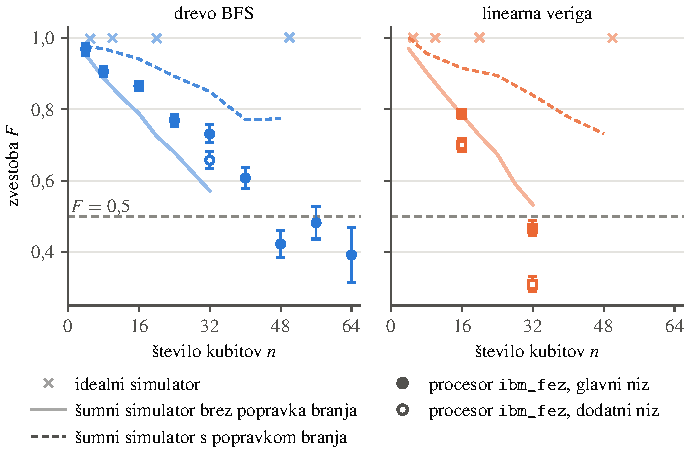
\includegraphics{zvestoba_n.pdf}
\caption{Zvestoba $F$ v odvisnosti od števila kubitov $n$ za drevo BFS in linearno verigo v konfiguraciji (i). Črte napak so $\pm 2\sigma$; točka, katere črta leži v celoti nad $F = 0{,}5$, izpolnjuje merilo $F - 2\sigma > 0{,}5$ za pristno večdelno prepletenost.}
\label{g30:fig:zvestoba}
\end{figure}

\begin{table}[htbp]
\caption{Zvestoba $F \pm \sigma$ na procesorju \texttt{ibm\_fez} po konfiguracijah blaženja napak. Krepko so označene vrednosti s $F - 2\sigma > 0{,}5$. Vrednosti (iv) so ocene z ekstrapolacijo.}
\label{g30:tab:rezultati}
\centering
% samodejno ustvari koda/grafi.py, ne urejaj rocno
\setlength{\aboverulesep}{0pt}
\setlength{\belowrulesep}{0pt}
\renewcommand{\arraystretch}{1.2}
\begin{tabular*}{\textwidth}{|@{}>{\hspace{5pt}}l@{\hspace{5pt}}|@{}>{\hspace{5pt}}l@{\hspace{5pt}}|@{}>{\hspace{5pt}}r@{\extracolsep{\fill}\hspace{5pt}}cccc<{\hspace{5pt}}@{\extracolsep{0pt}}|}
\toprule
Oblika & Niz & $n$ & (i) & (ii) & (iii) & (iv) \\
\midrule
\multirow{10}{*}{drevo} & \multirow{1}{*}{testni} & 4 & {\boldmath\bfseries 0,968 $\pm$ 0,008} & {\boldmath\bfseries 0,970 $\pm$ 0,007} & {\boldmath\bfseries 0,945 $\pm$ 0,009} & 0,950 $\pm$ 0,012 \\
\cline{2-7}
 & \multirow{8}{*}{glavni} & 8 & {\boldmath\bfseries 0,905 $\pm$ 0,007} & {\boldmath\bfseries 0,883 $\pm$ 0,007} & {\boldmath\bfseries 0,896 $\pm$ 0,007} & 0,912 $\pm$ 0,008 \\
 &  & 16 & {\boldmath\bfseries 0,865 $\pm$ 0,007} & {\boldmath\bfseries 0,790 $\pm$ 0,008} & {\boldmath\bfseries 0,798 $\pm$ 0,007} & 0,828 $\pm$ 0,009 \\
 &  & 24 & {\boldmath\bfseries 0,769 $\pm$ 0,008} & {\boldmath\bfseries 0,706 $\pm$ 0,009} & {\boldmath\bfseries 0,643 $\pm$ 0,009} & 0,705 $\pm$ 0,015 \\
 &  & 32 & {\boldmath\bfseries 0,731 $\pm$ 0,013} & {\boldmath\bfseries 0,572 $\pm$ 0,012} & {\boldmath\bfseries 0,548 $\pm$ 0,013} & 0,553 $\pm$ 0,016 \\
 &  & 40 & {\boldmath\bfseries 0,607 $\pm$ 0,015} & 0,476 $\pm$ 0,018 & 0,435 $\pm$ 0,020 & 0,382 \\
 &  & 48 & 0,422 $\pm$ 0,019 & -- & -- & -- \\
 &  & 56 & 0,482 $\pm$ 0,023 & -- & -- & -- \\
 &  & 64 & 0,392 $\pm$ 0,038 & -- & -- & -- \\
\cline{2-7}
 & \multirow{1}{*}{dodatni} & 32 & {\boldmath\bfseries 0,657 $\pm$ 0,012} & 0,473 $\pm$ 0,012 & -- & -- \\
\midrule
\multirow{4}{*}{veriga} & \multirow{2}{*}{glavni} & 16 & {\boldmath\bfseries 0,787 $\pm$ 0,007} & -- & -- & -- \\
 &  & 32 & 0,467 $\pm$ 0,011 & -- & -- & -- \\
\cline{2-7}
 & \multirow{2}{*}{dodatni} & 16 & {\boldmath\bfseries 0,700 $\pm$ 0,009} & {\boldmath\bfseries 0,629 $\pm$ 0,009} & 0,502 $\pm$ 0,014 & -- \\
 &  & 32 & 0,310 $\pm$ 0,010 & 0,174 $\pm$ 0,009 & 0,103 $\pm$ 0,009 & -- \\
\bottomrule
\end{tabular*}

\end{table}

\runinhead{Blaženje napak.} Iz Tabele~\ref{g30:tab:rezultati} je razvidno, da sta razklapljanje in sukanje zvestobo drevesa pri $n \geq 16$ znižala, meja pa je padla na največ 32 kubitov (Tabela~\ref{g30:tab:meje}). Pri $n = 40$ je razklapljanje vsoto populacij znižalo z $0{,}59$ na $0{,}41$, koherenco pa le z $0{,}62$ na $0{,}54$ (Slika~\ref{g30:fig:konfiguracije}). Konfiguracije (i)--(iii) so porabile enako procesorskega časa, po \SI{64}{\second}, konfiguracija (iv) pa \SI{123}{\second} (Tabela~\ref{g30:tab:meje}).

\begin{figure}[htbp]
\centering
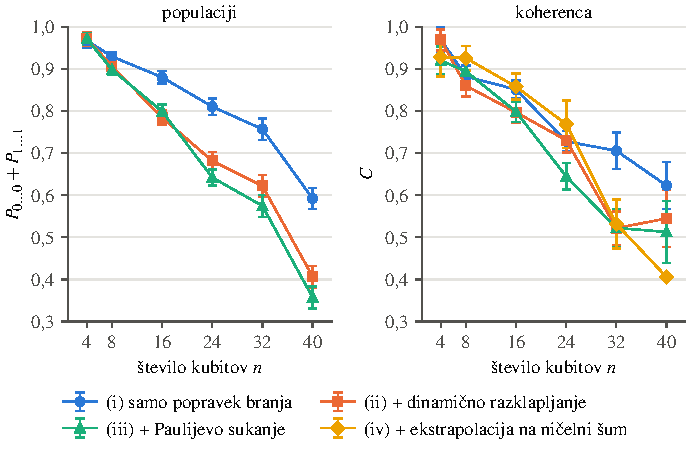
\includegraphics{konfiguracije.pdf}
\caption{Vsota populacij $P_{0\ldots0} + P_{1\ldots1}$ (levo) in koherenca $C$ (desno) za drevo BFS na procesorju po konfiguracijah blaženja napak. Črte napak so $\pm 2\sigma$. Konfiguracija (iv) ima populaciji iz (iii), zato je levo ni.}
\label{g30:fig:konfiguracije}
\end{figure}

\begin{table}[htbp]
\caption{Meja $n_{\mathrm{max}}$, največji izmerjeni $n$ s $F - 2\sigma > 0{,}5$, in procesorski čas $t_{\mathrm{QPU}}$ nalog Sampler in Estimator v glavnem nizu (drevo pri $n = 8$ do 40, veriga pri $n = 16$ in 32). Poševno zapisana meja je le zgornja, ker ponovljena meritev pri tem $n$ prepletenosti ni potrdila.}
\label{g30:tab:meje}
\centering
% samodejno ustvari koda/grafi.py, ne urejaj rocno
\setlength{\aboverulesep}{0pt}
\setlength{\belowrulesep}{0pt}
\renewcommand{\arraystretch}{1.2}
\begin{tabular}{|@{}>{\hspace{5pt}}l@{\hspace{5pt}}|@{}>{\hspace{5pt}}l@{\hspace{5pt}}|@{}>{\hspace{5pt}}c@{\hspace{5pt}}|@{}>{\hspace{5pt}}c@{\hspace{5pt}}|}
\toprule
Oblika & Konf. & $n_{\mathrm{max}}$ & $t_{\mathrm{QPU}}$ [\si{\second}] \\
\midrule
\multirow{4}{*}{drevo} & (i) & 40 & 64 \\
 & (ii) & \textit{32} & 64 \\
 & (iii) & 32 & 64 \\
 & (iv) & -- & 123 \\
\midrule
veriga & (i) & 16 & 25 \\
\bottomrule
\end{tabular}

\end{table}


\section{Razprava}
\label{g30:sec:razprava}

\runinhead{Odgovor na raziskovalno vprašanje.} Procesor \texttt{ibm\_fez} je stanje GHZ s pristno večdelno prepletenostjo pripravil na 40 kubitih z drevesom BFS in samim popravkom branja, z verigo pa na 16 kubitih (Tabela~\ref{g30:tab:meje}). Razklapljanje in sukanje sta mejo znižala na največ 32 kubitov; za (ii) lahko trdimo le, da meja ne presega 32 kubitov, ker ponovljena meritev pri $n = 32$ prepletenosti ni potrdila. Vse meje so rezultat posameznih zagonov: rezerva pri $n = 40$, $F - 0{,}5 = 0{,}107$, je primerljiva z razlikami med nizoma pri isti konfiguraciji, ki znašajo do $0{,}157$.

\runinhead{Primerjava s hipotezo in literaturo.} Napoved, da bo meja s samim popravkom branja 15--25 kubitov, je bila preveč pesimistična, napoved, da bo drevo preseglo verigo, pa se je potrdila. Napoved, da bosta razklapljanje in sukanje mejo povečala za vsaj \SI{30}{\percent} za ceno večkratnega procesorskega časa, je ovržena v obeh delih: meja se je znižala, procesorski čas pa se ni povečal. Ekstrapolacija je ocenjeno koherenco povečala le do $n = 24$. Naša meja je nad 32 kubiti, največjo velikostjo, ki so jo brez detekcije napak preizkusili Kam in sod.~\cite{g30:kam2024}, in pod 120 kubiti, doseženimi z detekcijo napak in post-selekcijo~\cite{g30:bigcats2025}; postavitve poskusov se razlikujejo, zato števila niso neposredno primerljiva.

\runinhead{Oblika vezja.} Obliki imata enako število vrat CZ in pri $n = 32$ skoraj enake vsote napak izbranih kubitov (napak CZ $0{,}08$ pri obeh, napak branja $0{,}41$ pri verigi in $0{,}44$ pri drevesu, \texttt{koda/pregled\_vezij.csv}). Razlikujeta se v času, ko kubiti po svojih prvih vratih mirujejo: po časovnem razvrščanju vezij, kot so tekla na procesorju, kubit v verigi pri $n = 32$ v povprečju miruje \SI{1,38}{\micro\second}, v drevesu pa \SI{0,17}{\micro\second}. Šumni model v Aerju mirovanju ne pripiše napake, ker ga prevedeno vezje ne vsebuje kot navodila, zato smo vezja v ločenem zagonu simulirali še z eksplicitnimi zakasnitvami na mestih mirovanja. Zakasnitve so zvestobo verige pri $n = 32$ znižale z $0{,}55$ na $0{,}36$, drevesa pa le z $0{,}57$ na $0{,}53$, večinoma prek koherence. Razlika med oblikama se je tako povečala z $0{,}02$ na $0{,}17$, na procesorju pa je bila $0{,}264$; po velikosti je ne primerjamo, ker simulacija nima popravka branja in teče na drugih kubitih. Obliki se razlikujeta tudi v postopku izbire kubitov, zato vpliva oblike in izbire kubitov ne moremo povsem ločiti.

\runinhead{Razklapljanje in sukanje.} Razklapljanje ščiti relativno fazo mirujočih kubitov in je zato namenjeno koherenci, pri drevesu pa je zmanjšalo predvsem vsoto populacij, koherence pa pri nobenem $n$ ni izboljšalo za več od statistične negotovosti (Slika~\ref{g30:fig:konfiguracije}). Z dodatnim nizom smo preverili dve razlagi. Pri verigi, kjer kubiti mirujejo pet- do osemkrat dlje, je razklapljanje zvestobo prav tako znižalo, pri $n = 16$ s $0{,}700$ na $0{,}629$ in pri $n = 32$ z $0{,}310$ na $0{,}174$. Pri drevesu z $n = 32$ je bilo znižanje ob obrnjenem vrstnem redu $0{,}184$, ob prvotnem pa $0{,}159$. Znižanja zato ne pripisujemo vrstnemu redu nalog niti pomanjkanju mirovanja. Napake impulzov ga ne pojasnijo: če bi bile neodvisne in enake kalibracijskim napakam vrat X, bi pri drevesu z $n = 40$ vsoto populacij zmanjšale za približno \SI{4}{\percent}, izmerili pa smo \SI{31}{\percent}, in v vseh sedmih primerjavah pri $n \geq 16$ je izmerjena izguba sedem- do dvanajstkrat večja od te ocene. Sukanje je zvestobo verige znižalo še naprej, na $0{,}502$ pri $n = 16$ in $0{,}103$ pri $n = 32$; ker je (iii) vedno tekla za (ii), vpliva vrstnega reda tu ne moremo izključiti. Vzroka za obe znižanji ne poznamo; da je učinek razklapljanja odvisen od zaporedja in naprave, so pokazali Ezzell in sod.~\cite{g30:ezzell2023}.

\runinhead{Ekstrapolacija.} Ekstrapolirana koherenca je bila pri $n = 8$, 16 in 24 višja od izmerjene v (iii), pri $n = 24$ na primer $0{,}77$ proti $0{,}64$, pri $n = 32$ je bila razlika manjša od negotovosti, pri $n = 40$ pa je bila ocena $0{,}41$ nižja od $0{,}51$ iz (iii) in brez negotovosti. Koherence pri faktorjih ojačanja 1, 3 in 5 so bile pri $n = 40$ enake $0{,}37$, $0{,}10$ in $0{,}06$, zato upad ni linearen.

\runinhead{Omejitve.} Ekstrapolacijo smo izmerili le na drevesu, razklapljanje in sukanje na verigi le pri dveh vrednostih $n$, meja pa je zaradi korakov po 8 znana le na interval osmih kubitov. Vsako točko smo izmerili enkrat, zato negotovosti zajemajo le statistični šum znotraj naloge, razlike med nizoma pa so večje; pri verigi z $n = 32$ je bila v dodatnem nizu vsota napak CZ izbranih kubitov dvakrat večja ($0{,}165$ proti $0{,}082$). Izbira kubitov ne upošteva časov razpada, in od $n = 32$ naprej je bil v vsakem drevesu kubit s $T_2$ pod \SI{17}{\micro\second}.

\subsection{Kaj ni delovalo}
\label{g30:sec:neuspehi}

Glavni neuspeh je, da razklapljanja in sukanja, na katerih je temeljila hipoteza, pred glavnim nizom nismo preizkusili pri velikosti vezja, pri kateri bi lahko opazili njun učinek. Pri testni nalogi z $n = 4$ razklapljanje ni vstavilo nobenega impulza, zvestoba v (i) in (ii) pa je bila enaka, $0{,}968$ in $0{,}970$.

Drugi neuspeh je eksponentni model $F = a\,e^{-n/n_0}$, s katerim smo nameravali določiti mejo. Prilagojen točkam (i) do $n = 40$ seka $0{,}5$ pri $n = 61 \pm 2$, izmerjena zvestoba pa merila ne izpolni že pri $n = 48$; tudi prilagojen vsem točkam (i), torej z $n = 48$, 56 in 64 vred, seka $0{,}5$ šele pri $n = 56 \pm 1$. Model mejo precenjuje, zato smo uporabili največji izmerjeni $n$.

Tretji neuspeh je napoved šumnega simulatorja, po kateri smo izbrali razpon $n$ za glavni niz: ker model mirovanju ni pripisal napake, razlike med oblikama ni napovedal (odstavek \emph{Oblika vezja}).


\section{Zaključek}
\label{g30:sec:zakljucek}

Procesor \texttt{ibm\_fez} je z drevesom BFS in samim popravkom napak branja pripravil stanje GHZ s pristno večdelno prepletenostjo na 40 kubitih, z linearno verigo pa na 16; obe meji sta rezultat posameznih zagonov. Obliki imata enako število vrat, kubiti v verigi pa po prvih vratih mirujejo pet- do osemkrat dlje, in v simulaciji z zakasnitvami prav mirovanje loči verigo od drevesa. Razklapljanje in sukanje procesorskega časa nista podaljšala, a sta zvestobo v vseh naših primerjavah znižala, ekstrapolacija pa je porabo skoraj podvojila. Največjo mejo je na tej napravi dala osnovna konfiguracija.

Delo bi nadaljevali s ponovljenimi meritvami na različnih kubitih, z gostejšim vzorčenjem $n$ med 40 in 48, z izbiro kubitov, ki upošteva tudi čase razpada, in z iskanjem vzroka, zakaj razklapljanje stane več, kot napovedo kalibracijske napake vrat. Večji doseg bi verjetno zahteval detekcijo napak s post-selekcijo~\cite{g30:bigcats2025}.


\section*{Doprinosi avtorjev}

Veno Jakomin je zasnoval in implementiral vezji za pripravo stanja GHZ ter izbiro kubitov na grafu naprave, izvedel idealne in šumne simulacije z lastno izvedbo ekstrapolacije na ničelni šum ter napisal Razdelka~\ref{g30:sec:uvod} in~\ref{g30:sec:metode}.

Jure Pahor je naredil cevovod za oceno zvestobe iz populacij in paritetnih nihanj z negotovostmi (\texttt{zvestoba.py}, \texttt{procesor.py}), prileganje $F(n)$ in mejo $n_{\mathrm{max}}$ (\texttt{analiza.py}), ter naredil grafe in tabele za rezultate (\texttt{grafi.py}). 
V poročilu je napisal Razdelek~\ref{g30:sec:rezultati}, naredil nekaj popravkov in poenotil stil tabel.

Grega Potočnik je nastavil konfiguracije blaženja napak v Qiskit Runtime, izvedel testno nalogo in iz nje izpeljal napoved porabe procesorskega časa, napisal program za oddajo nalog s sprotnim beleženjem identifikatorjev, porabe in kalibracijskih podatkov, oddal vse naloge na procesor \texttt{ibm\_fez}, zasnoval in izvedel dodatna poskusa z razklapljanjem na verigi in z obrnjenim vrstnim redom konfiguracij, iz prevedenih vezij ovrednotil čas mirovanja in ceno razklapljanja ter napisal Razdelka~\ref{g30:sec:izvedba} in~\ref{g30:sec:neuspehi}.

\section*{Izjava o uporabi generativne umetne inteligence}

Pri delu smo uporabljali asistenta Claude (Anthropic) v okolju Claude Code za preverjanje kode in rezultatov ter za iskanje in pregled virov. Vse njegove ugotovitve smo preverili na podatkih in v virih; za vsebino poročila odgovarjamo avtorji.
